%TODO no numeri a lato del codice
\begin{frame}[t,plain]
\titlepage
\end{frame}

\begin{frame}{Steps}
	\begin{itemize}
		\item Calibration
		\item Unwarping
		\item Detection
		\item Path planning
		\item Dubins interpolation
		\item Localization
	\end{itemize}
\end{frame}

\begin{frame}[fragile]{But first Settings}	
	\texttt{Settings.xml}
\end{frame}

\begin{frame}[fragile]{Settings}	
	\begin{center}
		\includegraphics[width=\linewidth]{Immagini/settings.png}
	\vspace{1cm}
	\newline
	\href{https://icosac.github.io/LabRoboticsProject/html/class_settings.html#a4a464c938e96639861dc2deb773a2fb8}{Link to settings.hh}
	\end{center}
\end{frame}

\begin{frame}{Support objects – maths.hh}
	\begin{itemize}
		\item Angle: class to handle both RAD and DEG angles.
		\item Tuple: an extension of vector.
		\item Point2: a simple point in the cartesian plane, with useful functionalities.
		\item Configuration2: a \texttt{Point2} with an orientation as \texttt{Angle}. 
	\end{itemize}
\end{frame}
\begin{frame}[fragile]{maths.hh}
\begin{center}
	\href{https://icosac.github.io/LabRoboticsProject/html/maths_8hh.html}{\includegraphics[width=\linewidth]{Immagini/maths}}
\end{center}
\end{frame}

\begin{frame}[fragile]{Support objects – filter.hh}
Class attributes:
\begin{itemize}
	\item low$\_$h: Lower value for hue	
	\item low$\_$s: Lower value for saturation
	\item low$\_$v: Lower value for value
	\item high$\_$h: Higher value for hue
	\item high$\_$s: Higher value for saturation
	\item high$\_$v: Higher value for value
\end{itemize}
Class functions:
\begin{itemize}
	\item High();
	\item Low();
\end{itemize}
Each returns a \texttt{Scalar} with the correspondent values.
\end{frame}

\begin{frame}{Calibration}
	Given a set of pictures taken with a camera, the object of this step is to find the camera matrix $A$ and the distortion coefficients $\dot{d}$.\newline
	\vfill
	\[
		A=\begin{bmatrix}
			f_x&0&c_x\\
			0&f_y&c_y\\
			0&0&1\\
		\end{bmatrix}\qquad
		\begin{matrix}
			x_{distorted}=x\left(1+k_1r^2+k_2r^4+k_3r^6\right)\\
			y_{distorted}=y\left(1+k_1r^2+k_2r^4+k_3r^6\right)\\
			x_{distorted}=x+\left[2p_1xy+p_2\left(r^2+2x^2\right)\right]\\
			y_{distorted}=y+\left[p_1\left(r^2+2y^2\right)+2p_2xy\right]\\
			\dot{d}=(k_1, k_2, p_1, p_2, k_3)
		\end{matrix}
	\]
	\vfill
\end{frame}


\begin{frame}{Calibration}
	\begin{figure}[H]
		\begin{minipage}{0.48\linewidth}
			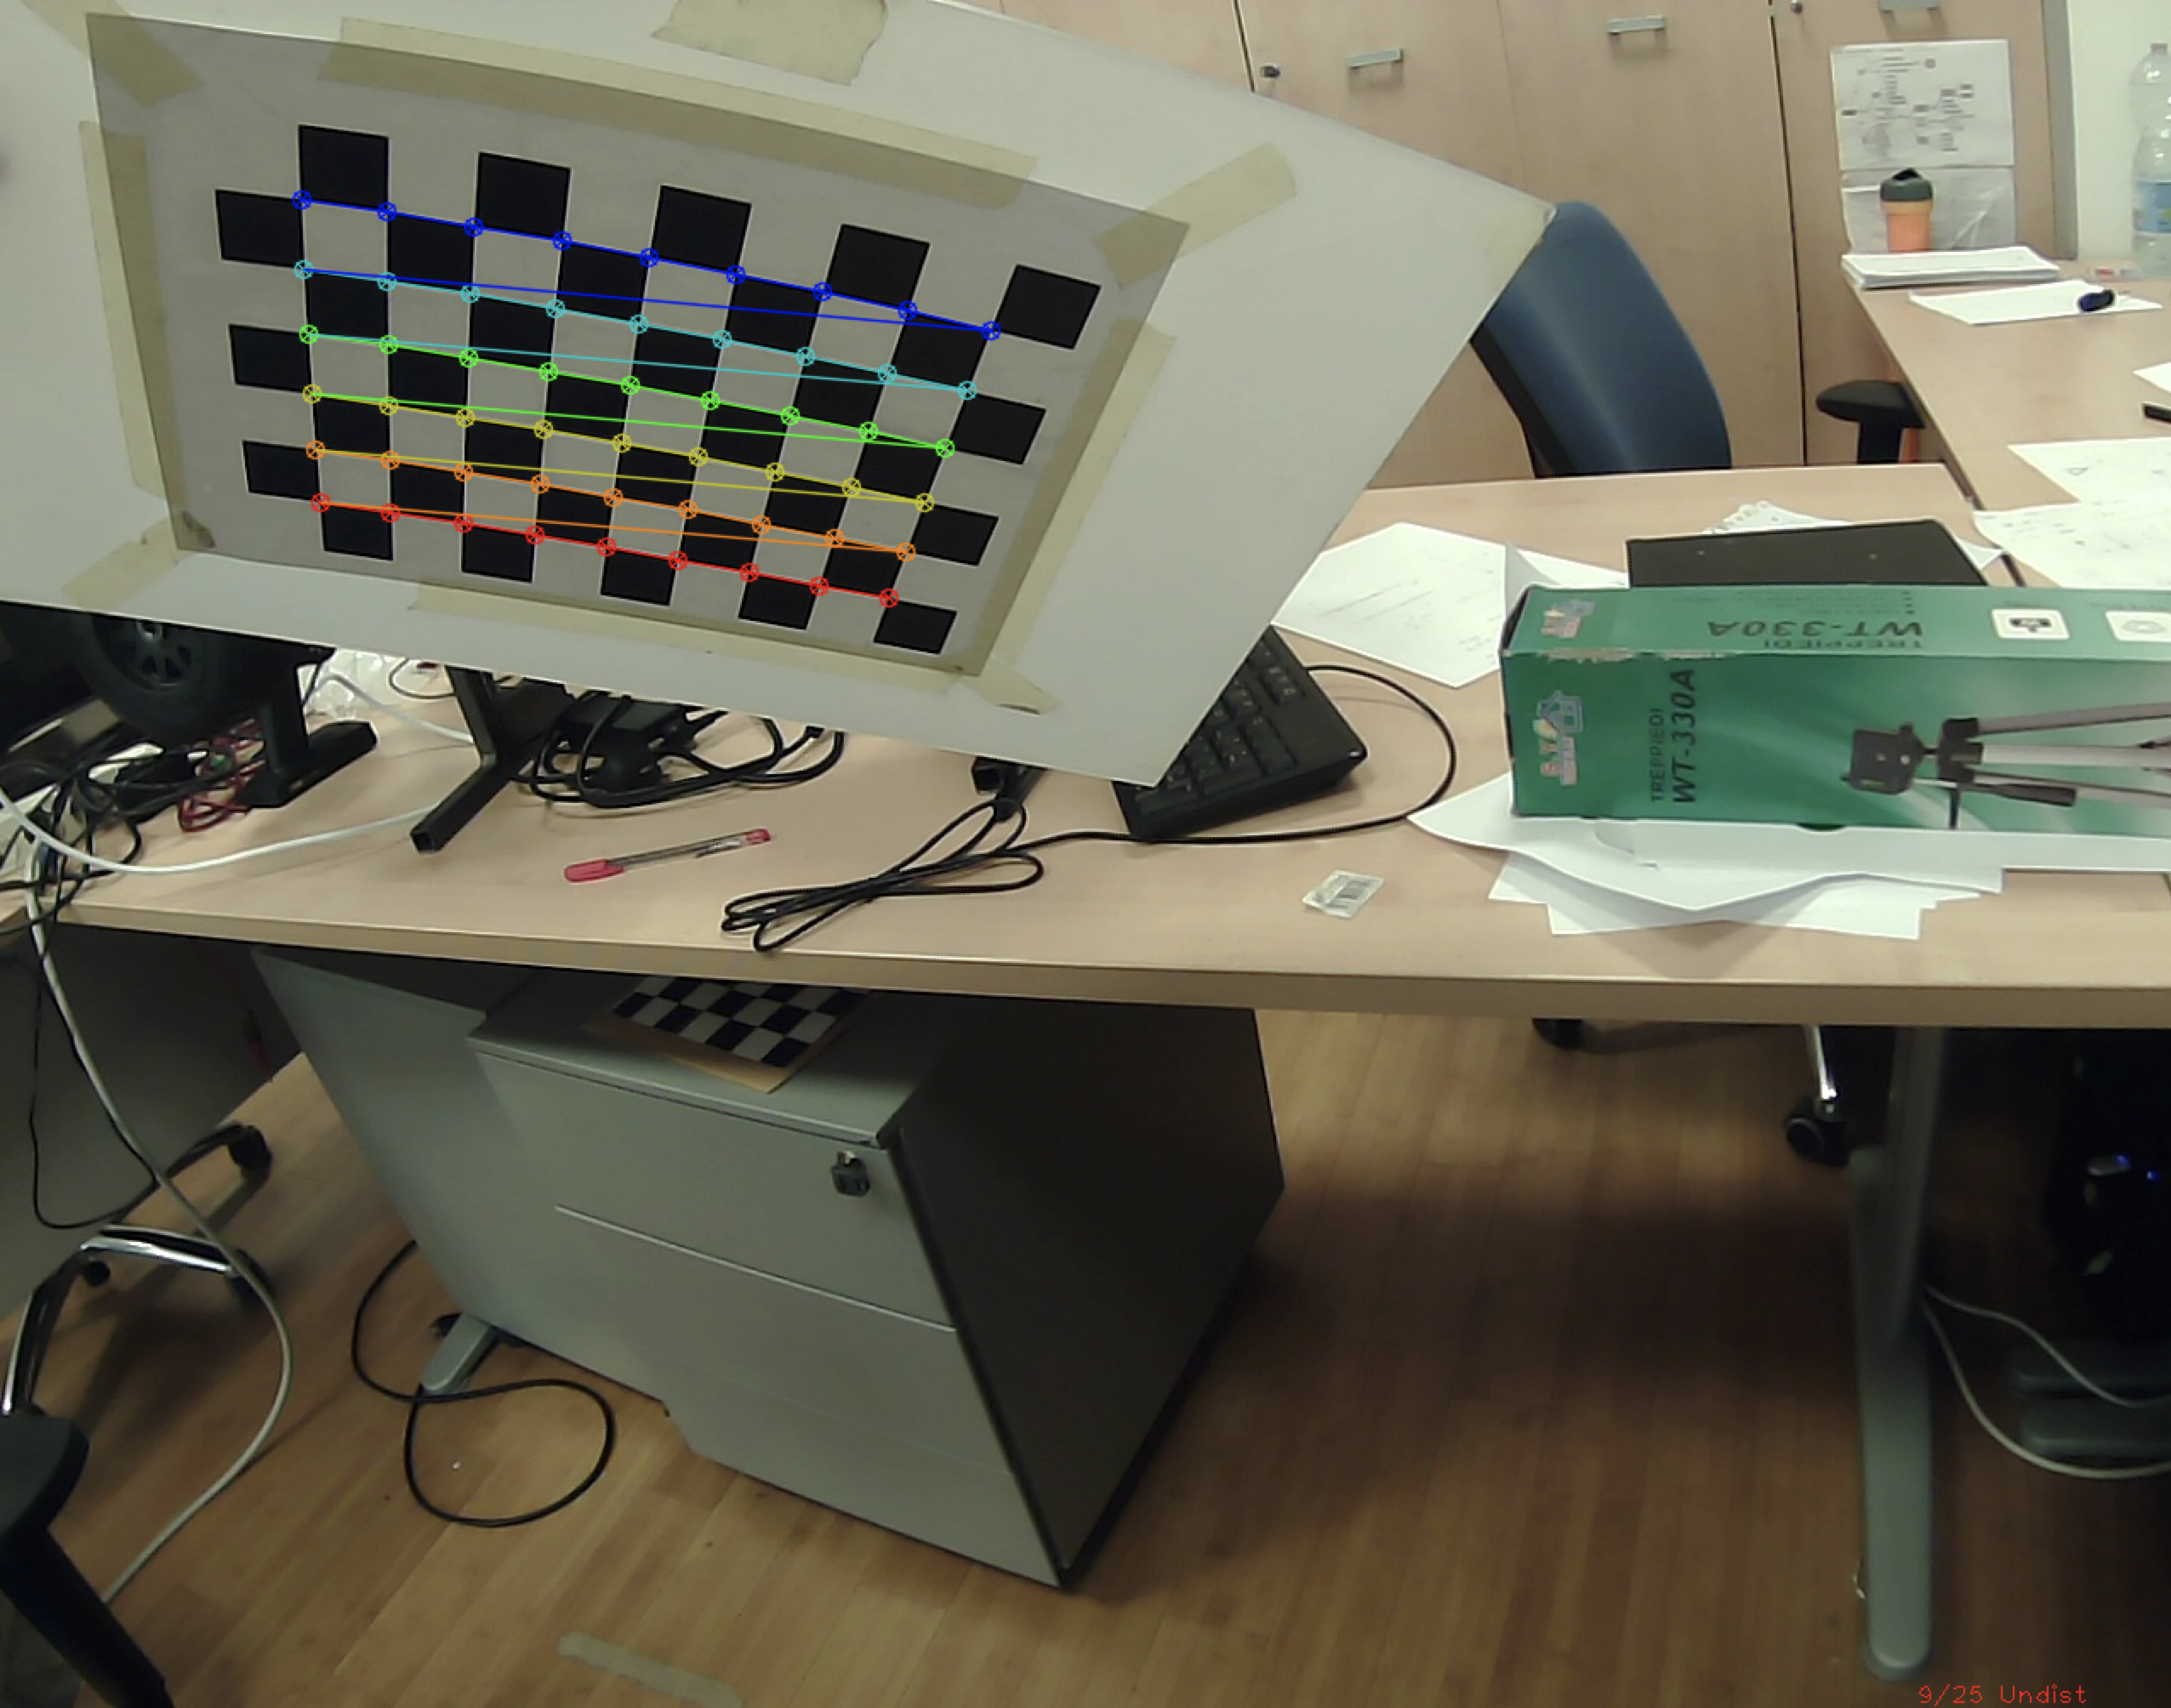
\includegraphics[width=\linewidth]{Immagini/Chessboard1}
		\end{minipage}
		\vspace{0.04\linewidth}
		\begin{minipage}{0.48\linewidth}
			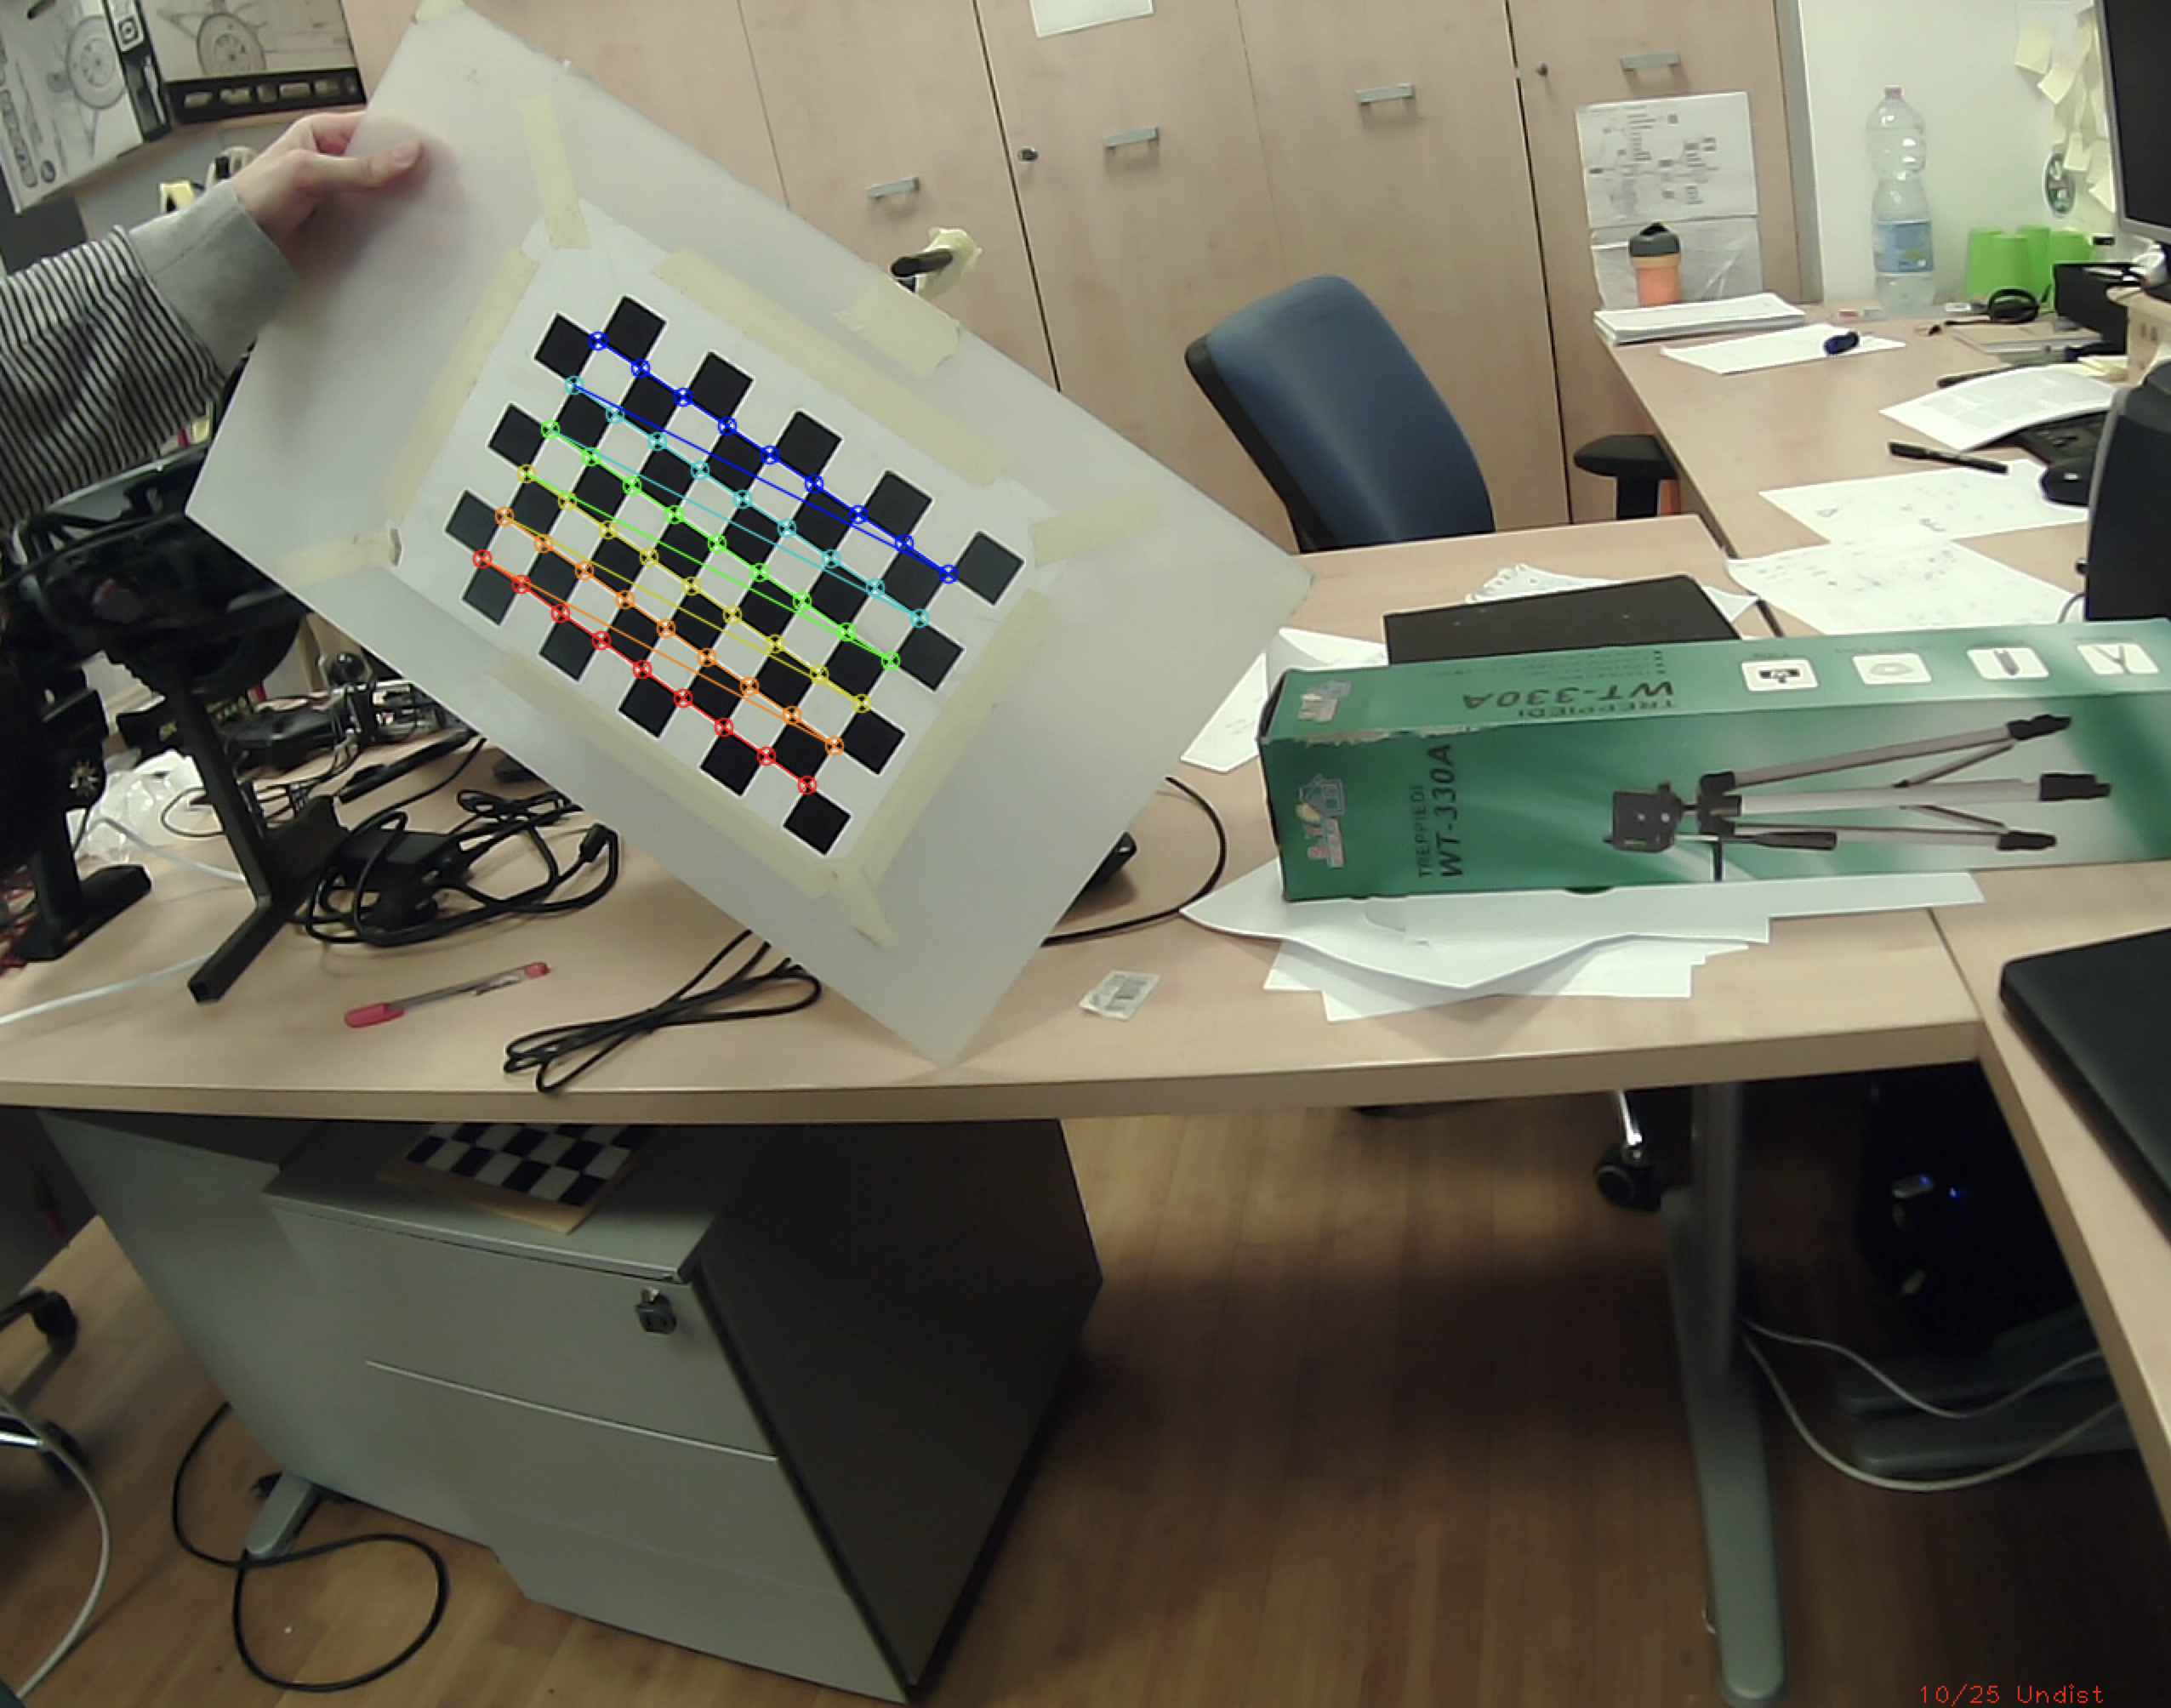
\includegraphics[width=\linewidth]{Immagini/Chessboard2}
		\end{minipage}
	\end{figure}
\end{frame}


\begin{frame}{Calibration}
	\begin{figure}[H]
		\begin{minipage}{0.48\linewidth}
			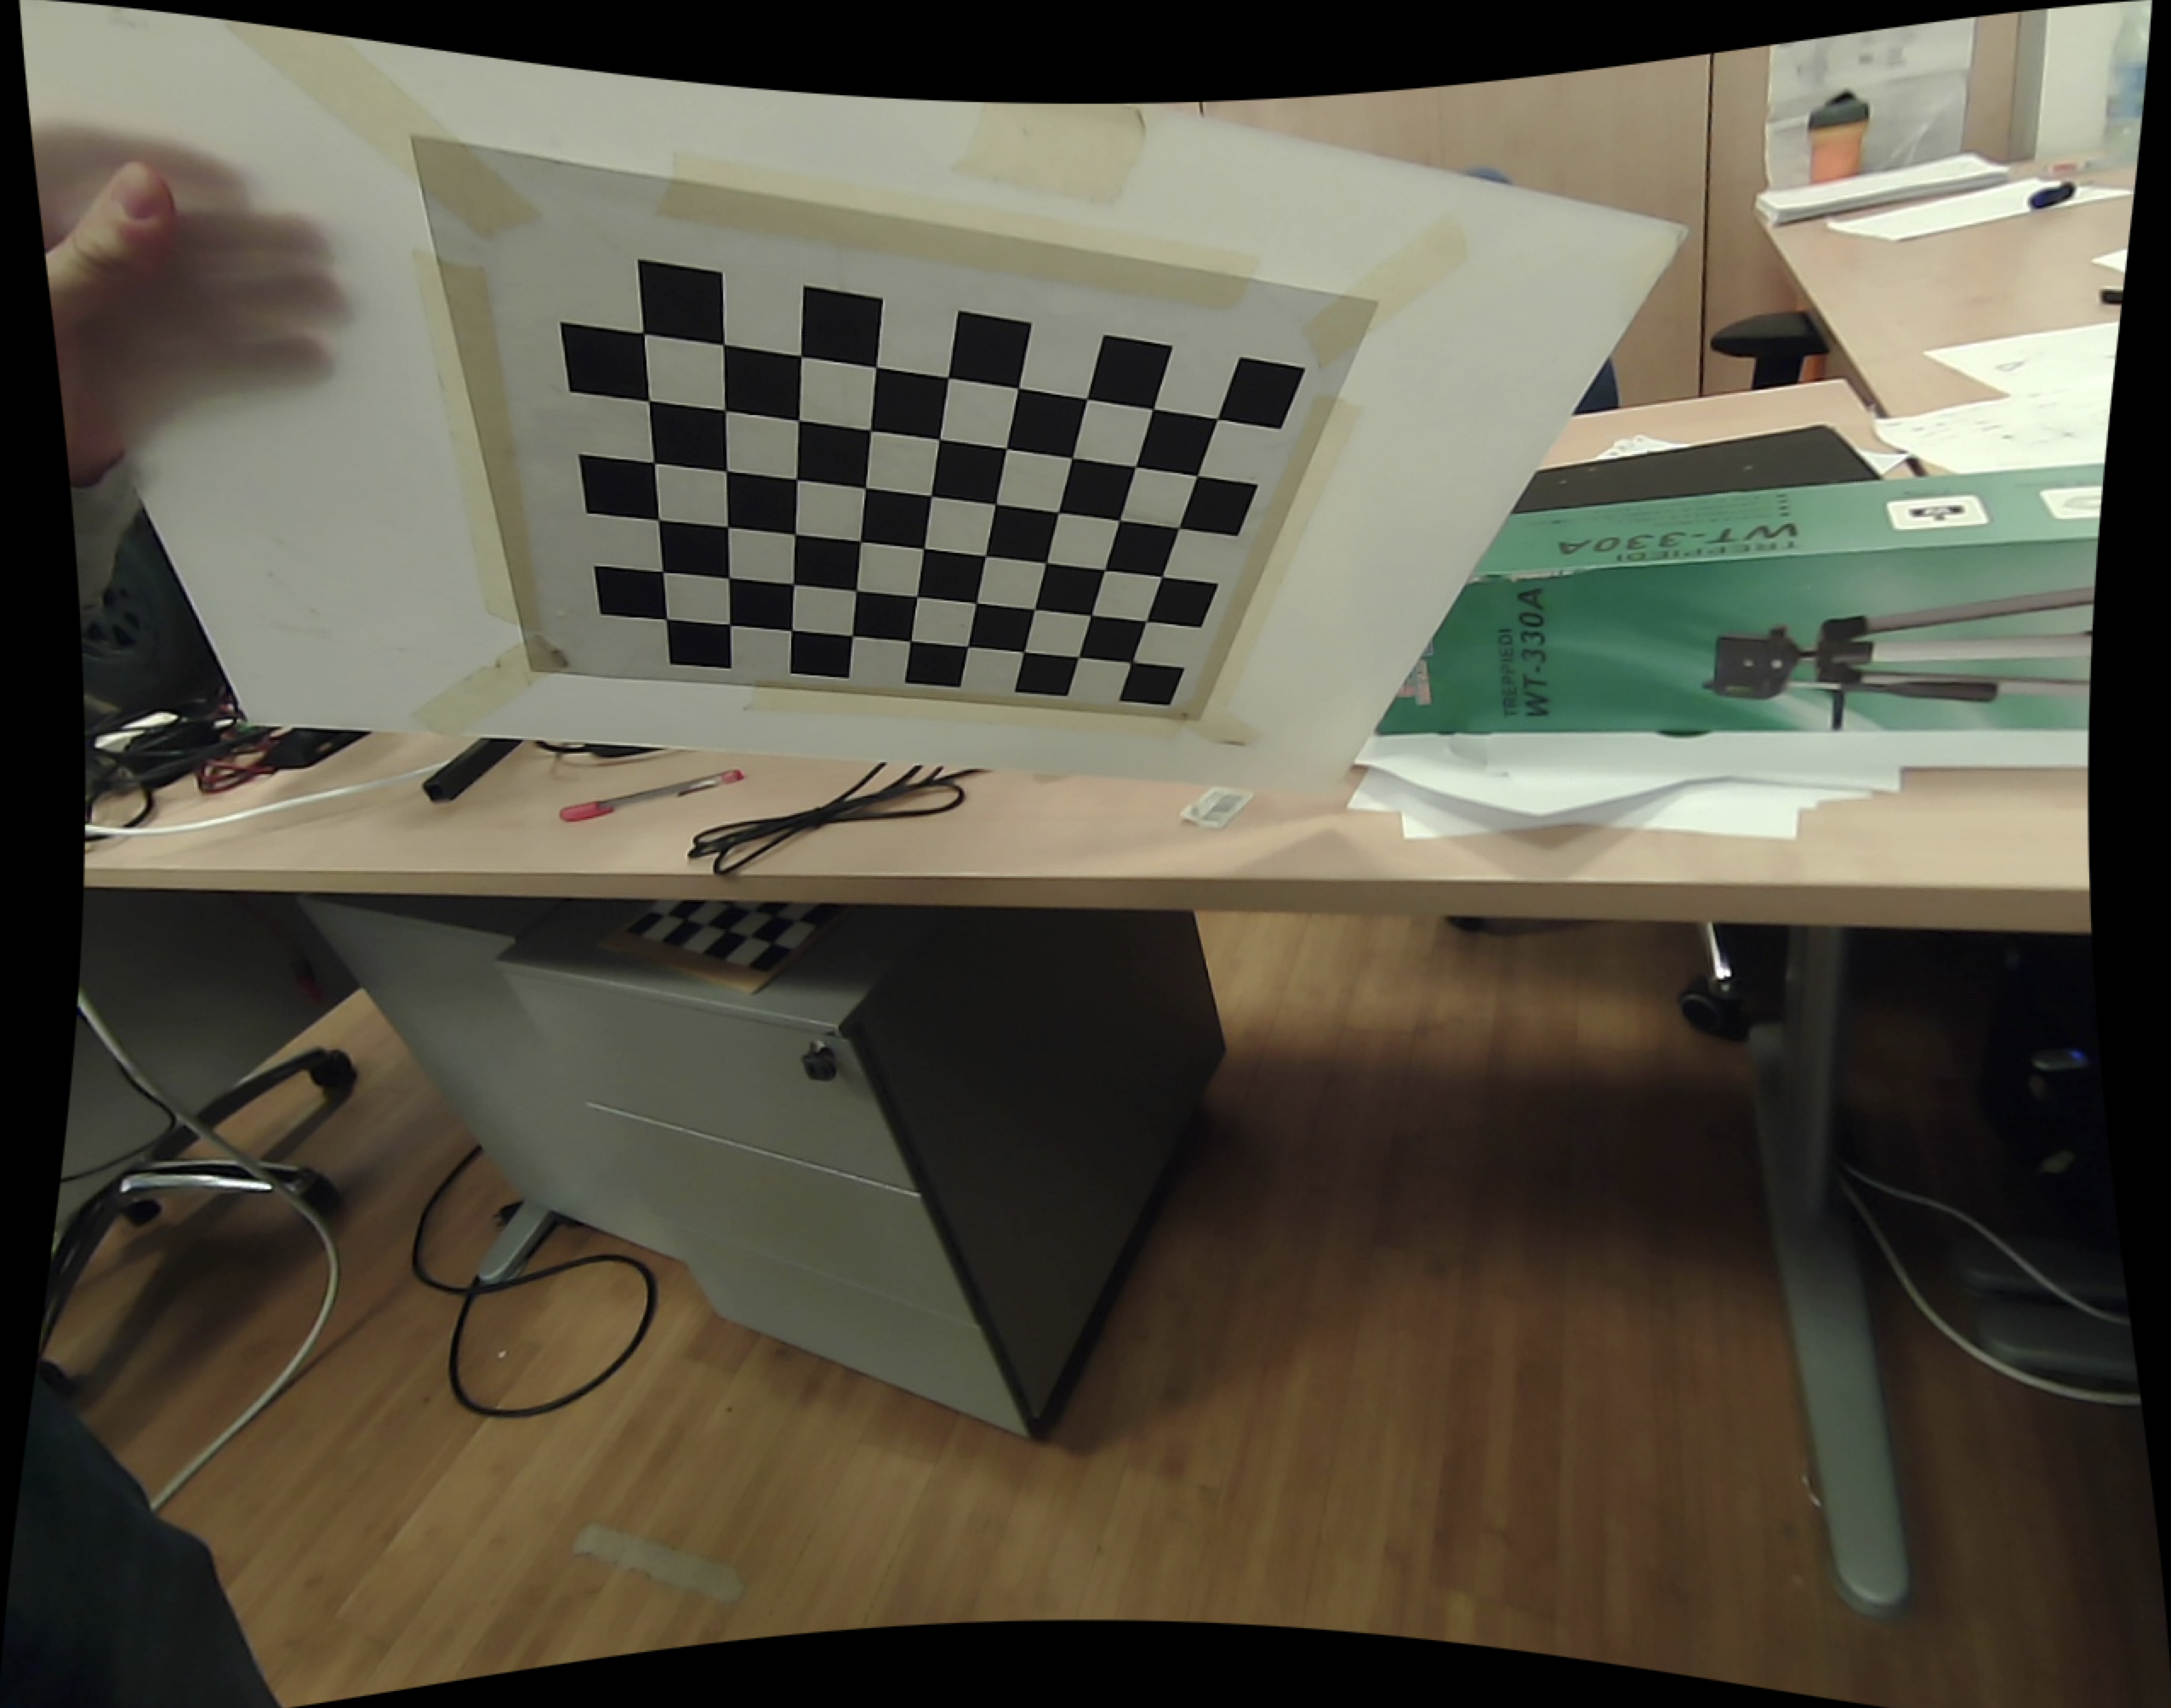
\includegraphics[width=\linewidth]{Immagini/Chessboard1Calibrated}
		\end{minipage}
		\vspace{0.04\linewidth}
		\begin{minipage}{0.48\linewidth}
			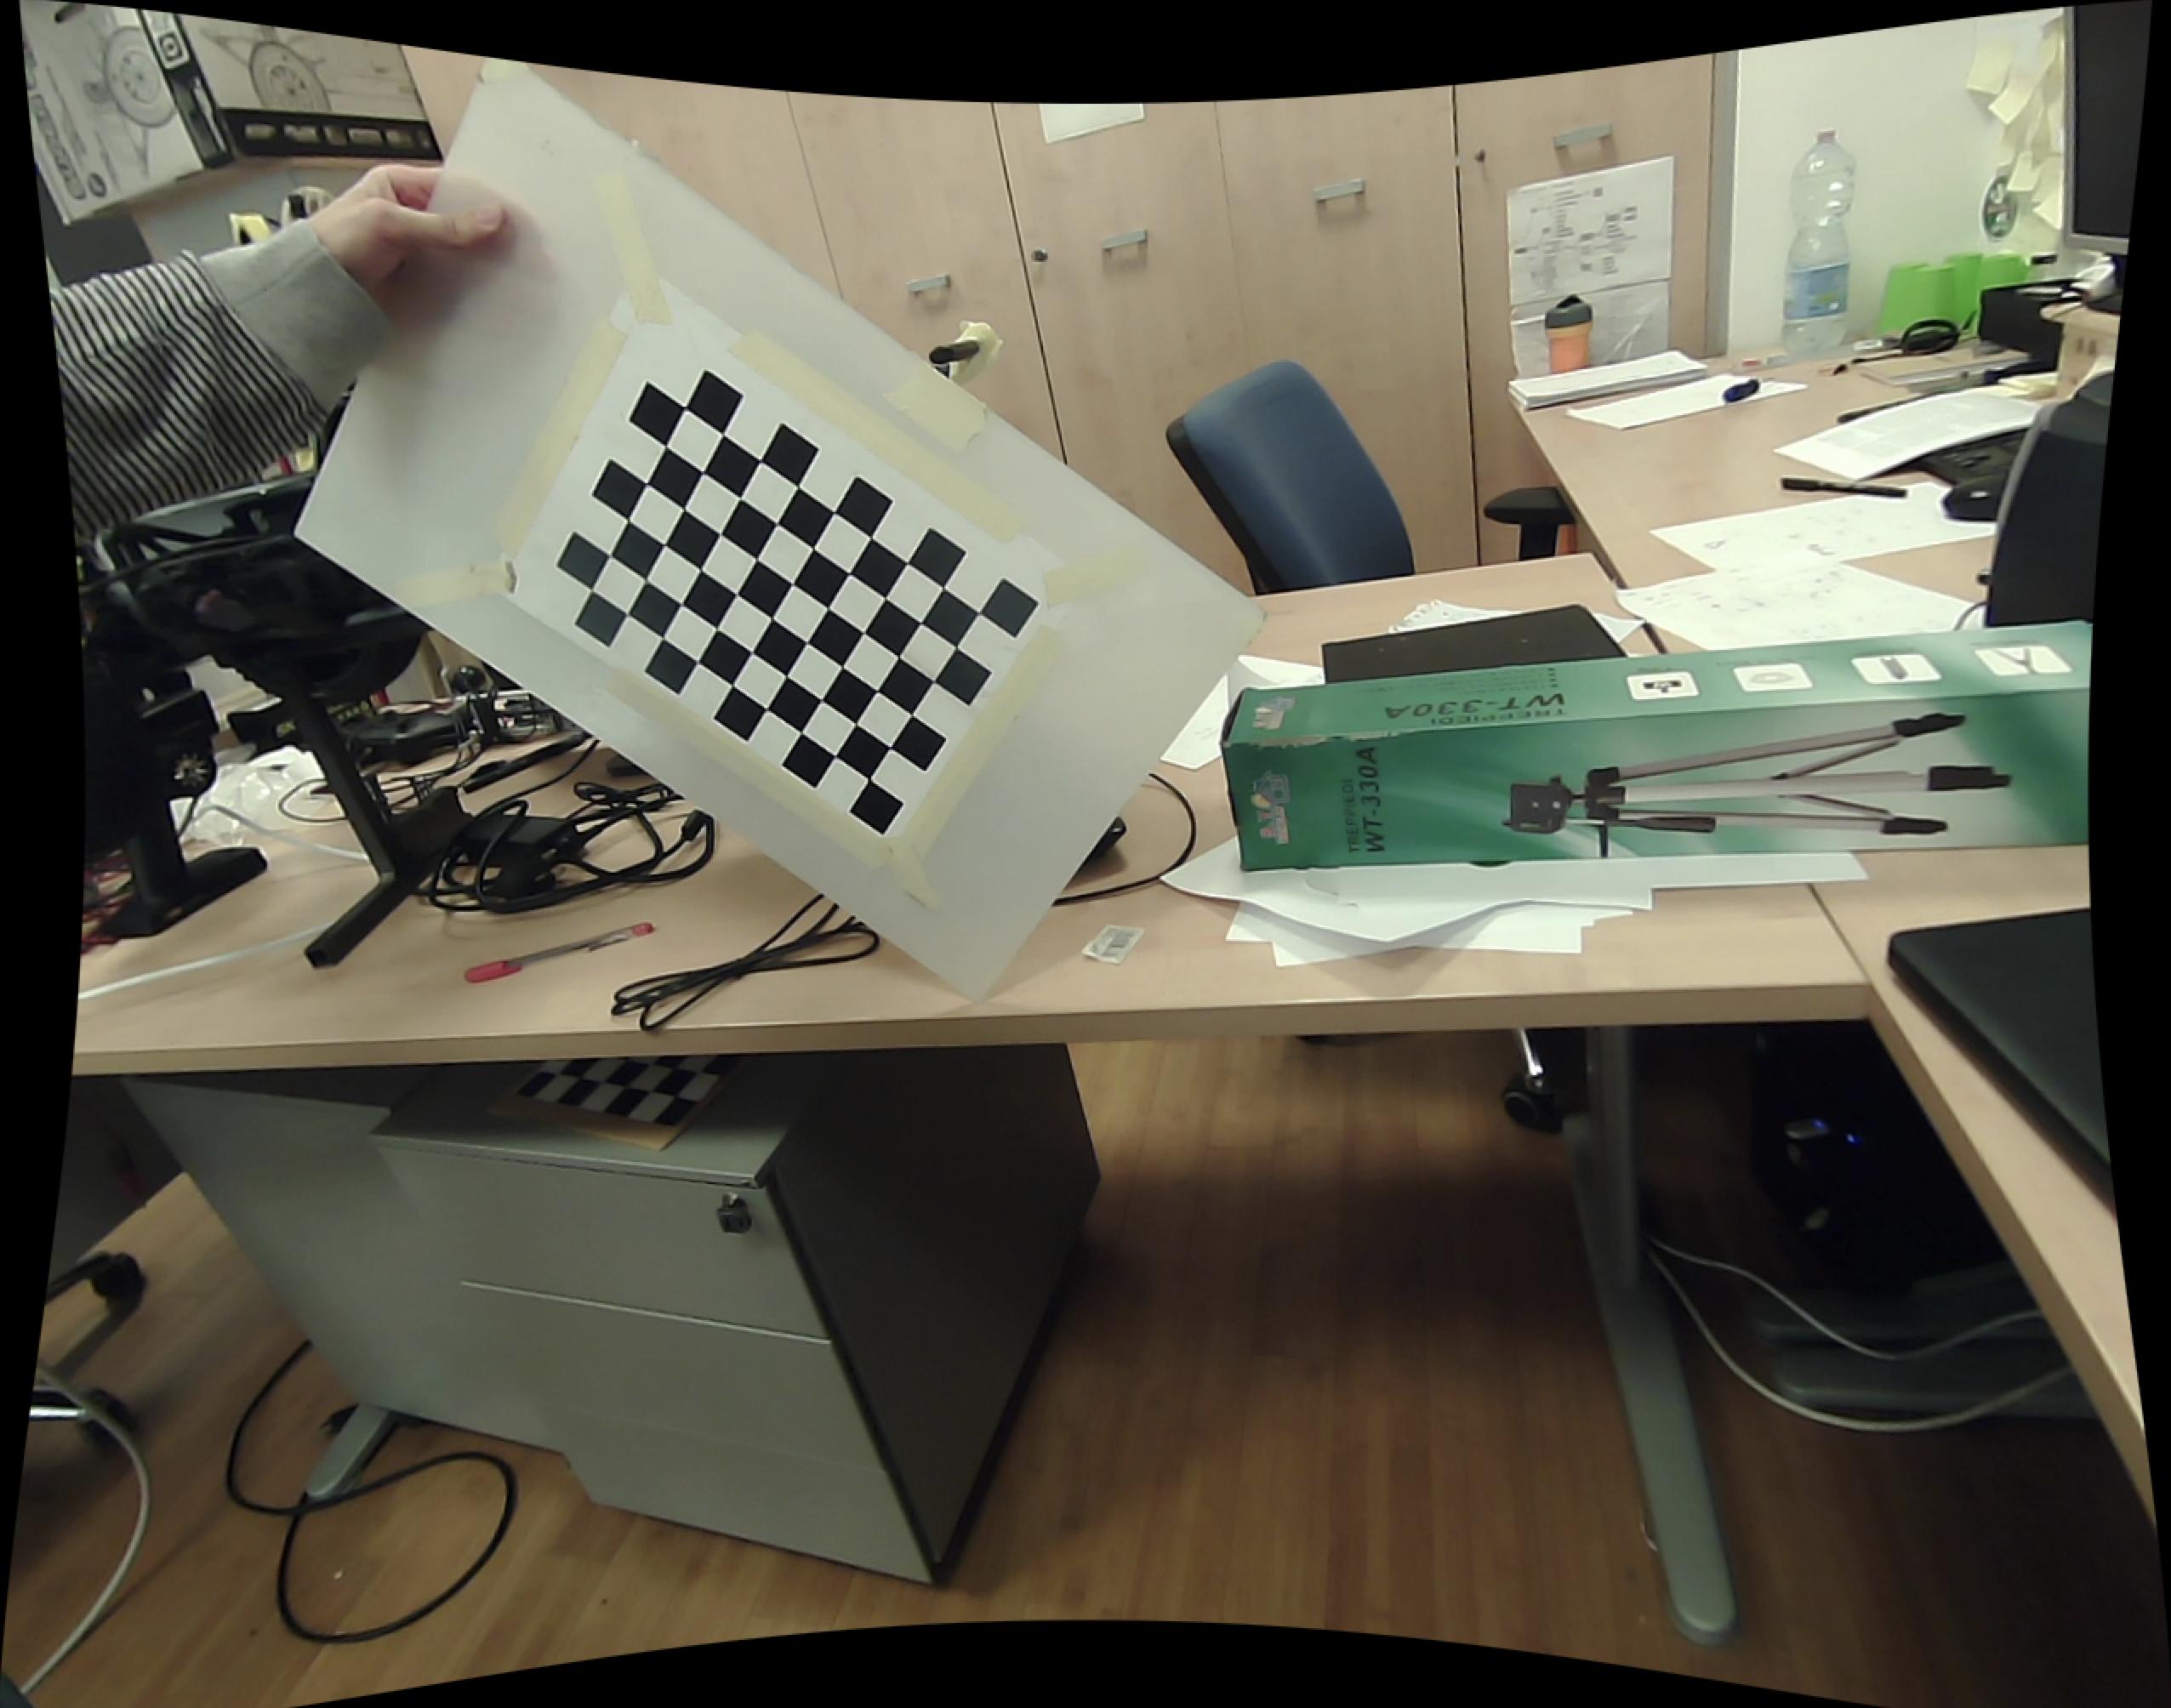
\includegraphics[width=\linewidth]{Immagini/Chessboard2Calibrated}
		\end{minipage}
	\end{figure}
	\stsize
	\[A=\begin{bmatrix}
		8.4247565095622963\times10^2 & 0 & 6.3709750745251142\times10^2\\
		0 & 8.4247565095622963\times10^2 & 4.9404840840221556\times10^2\\
		0 & 0 & 1
	\end{bmatrix}\]\[
	\dot{d}=(-2.5214446354851400\times10^{-1}, 7.2467634259951161\times10^{-2},\]\[-3.7212601356153754\times10^{-3}, 4.3313659139950872\times10^{-4}, 0)
	\]
\end{frame}

\begin{frame}[fragile]{Configure}
Function to change the filters if the result of their use doesn't look good.
\end{frame}

\begin{frame}[fragile]{Configure}
\begin{center}
\includegraphics[width=\linewidth]{Immagini/configure1}
\end{center}
\begin{center}
\includegraphics[width=\linewidth]{Immagini/configure2}
\end{center}
\end{frame}

\begin{frame}[fragile]{Configure}
\begin{figure}[H]
	\begin{minipage}{0.48\linewidth}
		\includegraphics[width=\linewidth]{Immagini/filterBlack}
	\end{minipage}
	\vspace{0.04\linewidth}
	\begin{minipage}{0.48\linewidth}
		\includegraphics[width=\linewidth]{Immagini/filterBlue}
	\end{minipage}
\end{figure}
\end{frame}

\begin{frame}[fragile]{Configure}
\begin{figure}[H]
	\begin{minipage}{0.48\linewidth}
		\includegraphics[width=\linewidth]{Immagini/filterRed}
	\end{minipage}
	\vspace{0.04\linewidth}
	\begin{minipage}{0.48\linewidth}
		\includegraphics[width=\linewidth]{Immagini/filterGreen}
	\end{minipage}
\end{figure}
\end{frame}

\begin{frame}[fragile]{Configure}
\begin{figure}[H]
	\begin{minipage}{0.48\linewidth}
		\includegraphics[width=\linewidth]{Immagini/filterRobot}
	\end{minipage}
	\vspace{0.07\linewidth}
	\begin{minipage}{0.45\linewidth}
		Once finished setting them up, the filters are saved in settings.xml and available during all the execution.
	\end{minipage}
\end{figure}
\end{frame}

\begin{frame}[fragile]{Unwarping}
Once the camera matrix and the distortion coefficients are known and the filters are nice, the next step is to focus on the target, that is the circuit, and then to “un-distort” it from this: 
	\begin{center}
		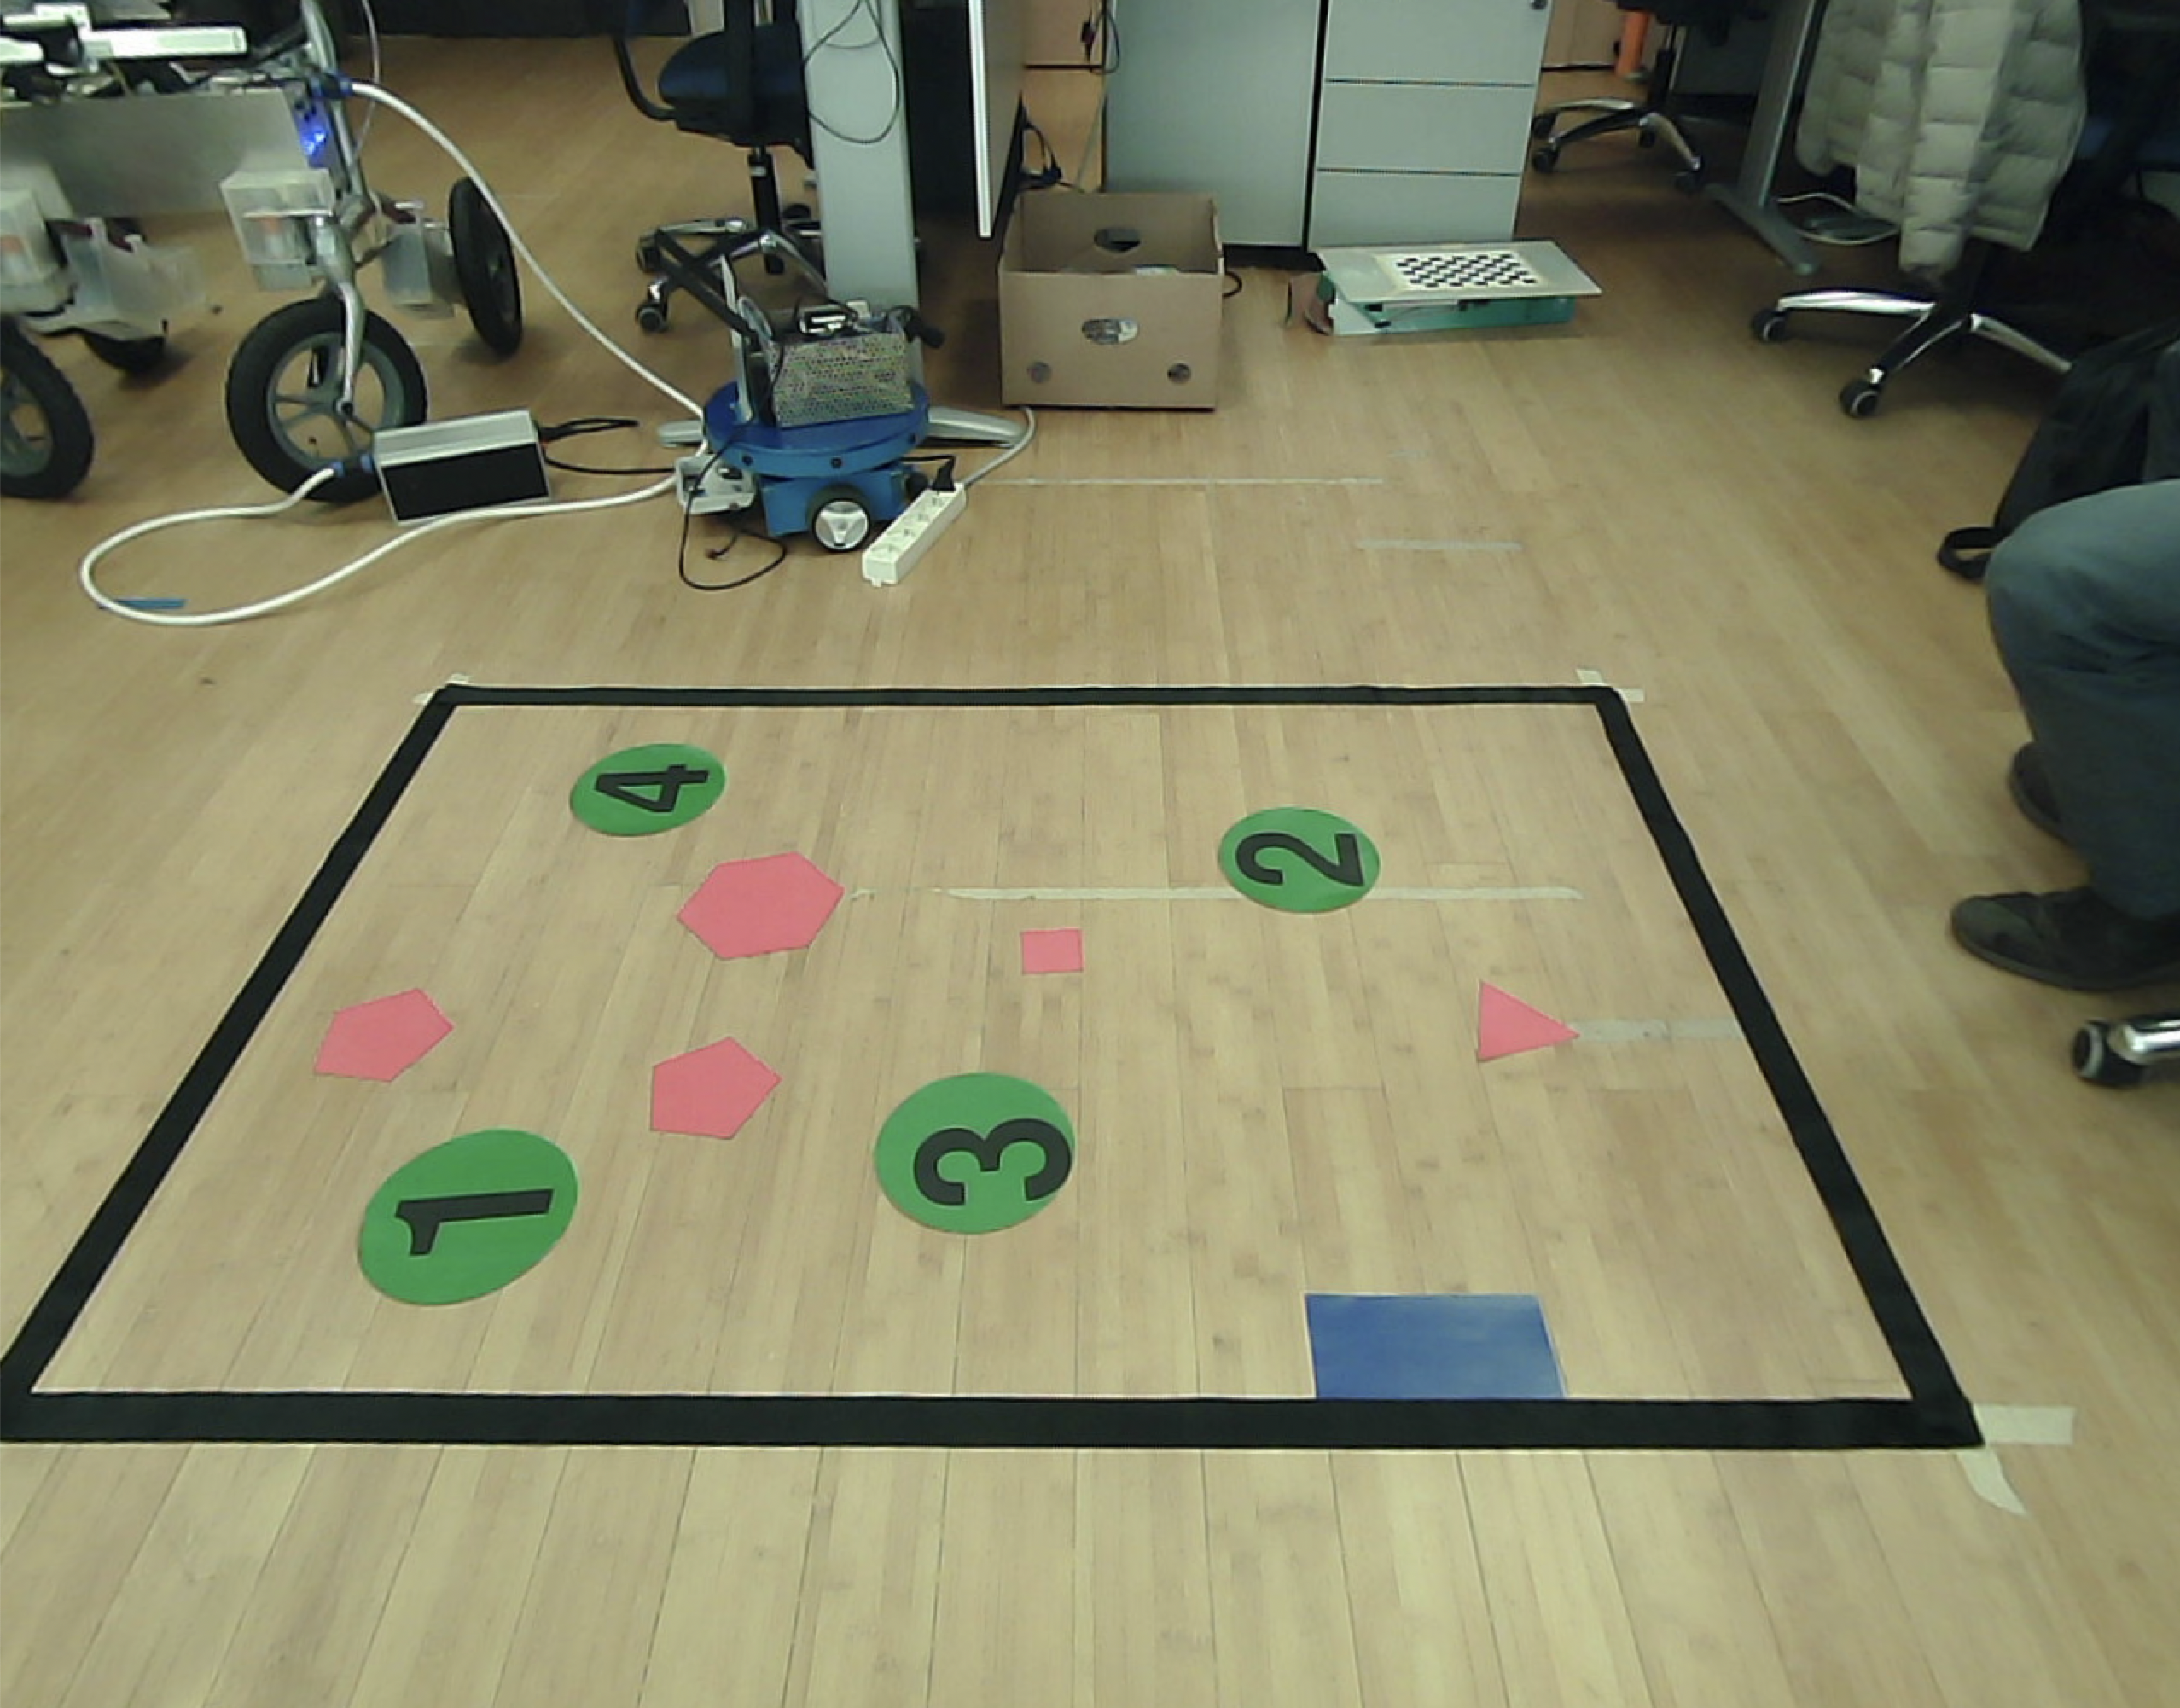
\includegraphics[scale=0.145]{Immagini/UNUndistort}
	\end{center}
\end{frame}

\begin{frame}[fragile]{Unwarping}
To this:
	\begin{center}
		\includegraphics[scale=0.18]{Immagini/Unwrapped.png}
	\end{center}
\end{frame}
%TODO change this images

\begin{frame}[fragile]{Unwarping}
	Straighten the image using the distortion coefficients. 
	\begin{center}
		\includegraphics[scale=0.15]{Immagini/Undistorted}	
	\end{center}
	\begin{minted}[fontsize=\stsize]{c++}
		loadCoefficients(calib_file, camera_matrix, dist_coeffs);
		undistort(or_img, fix_img, camera_matrix, dist_coeffs);
	\end{minted}
\end{frame}

\begin{frame}[fragile]{Unwarping}
	Then the image is converted from RGB to HSV.
	\begin{center}
		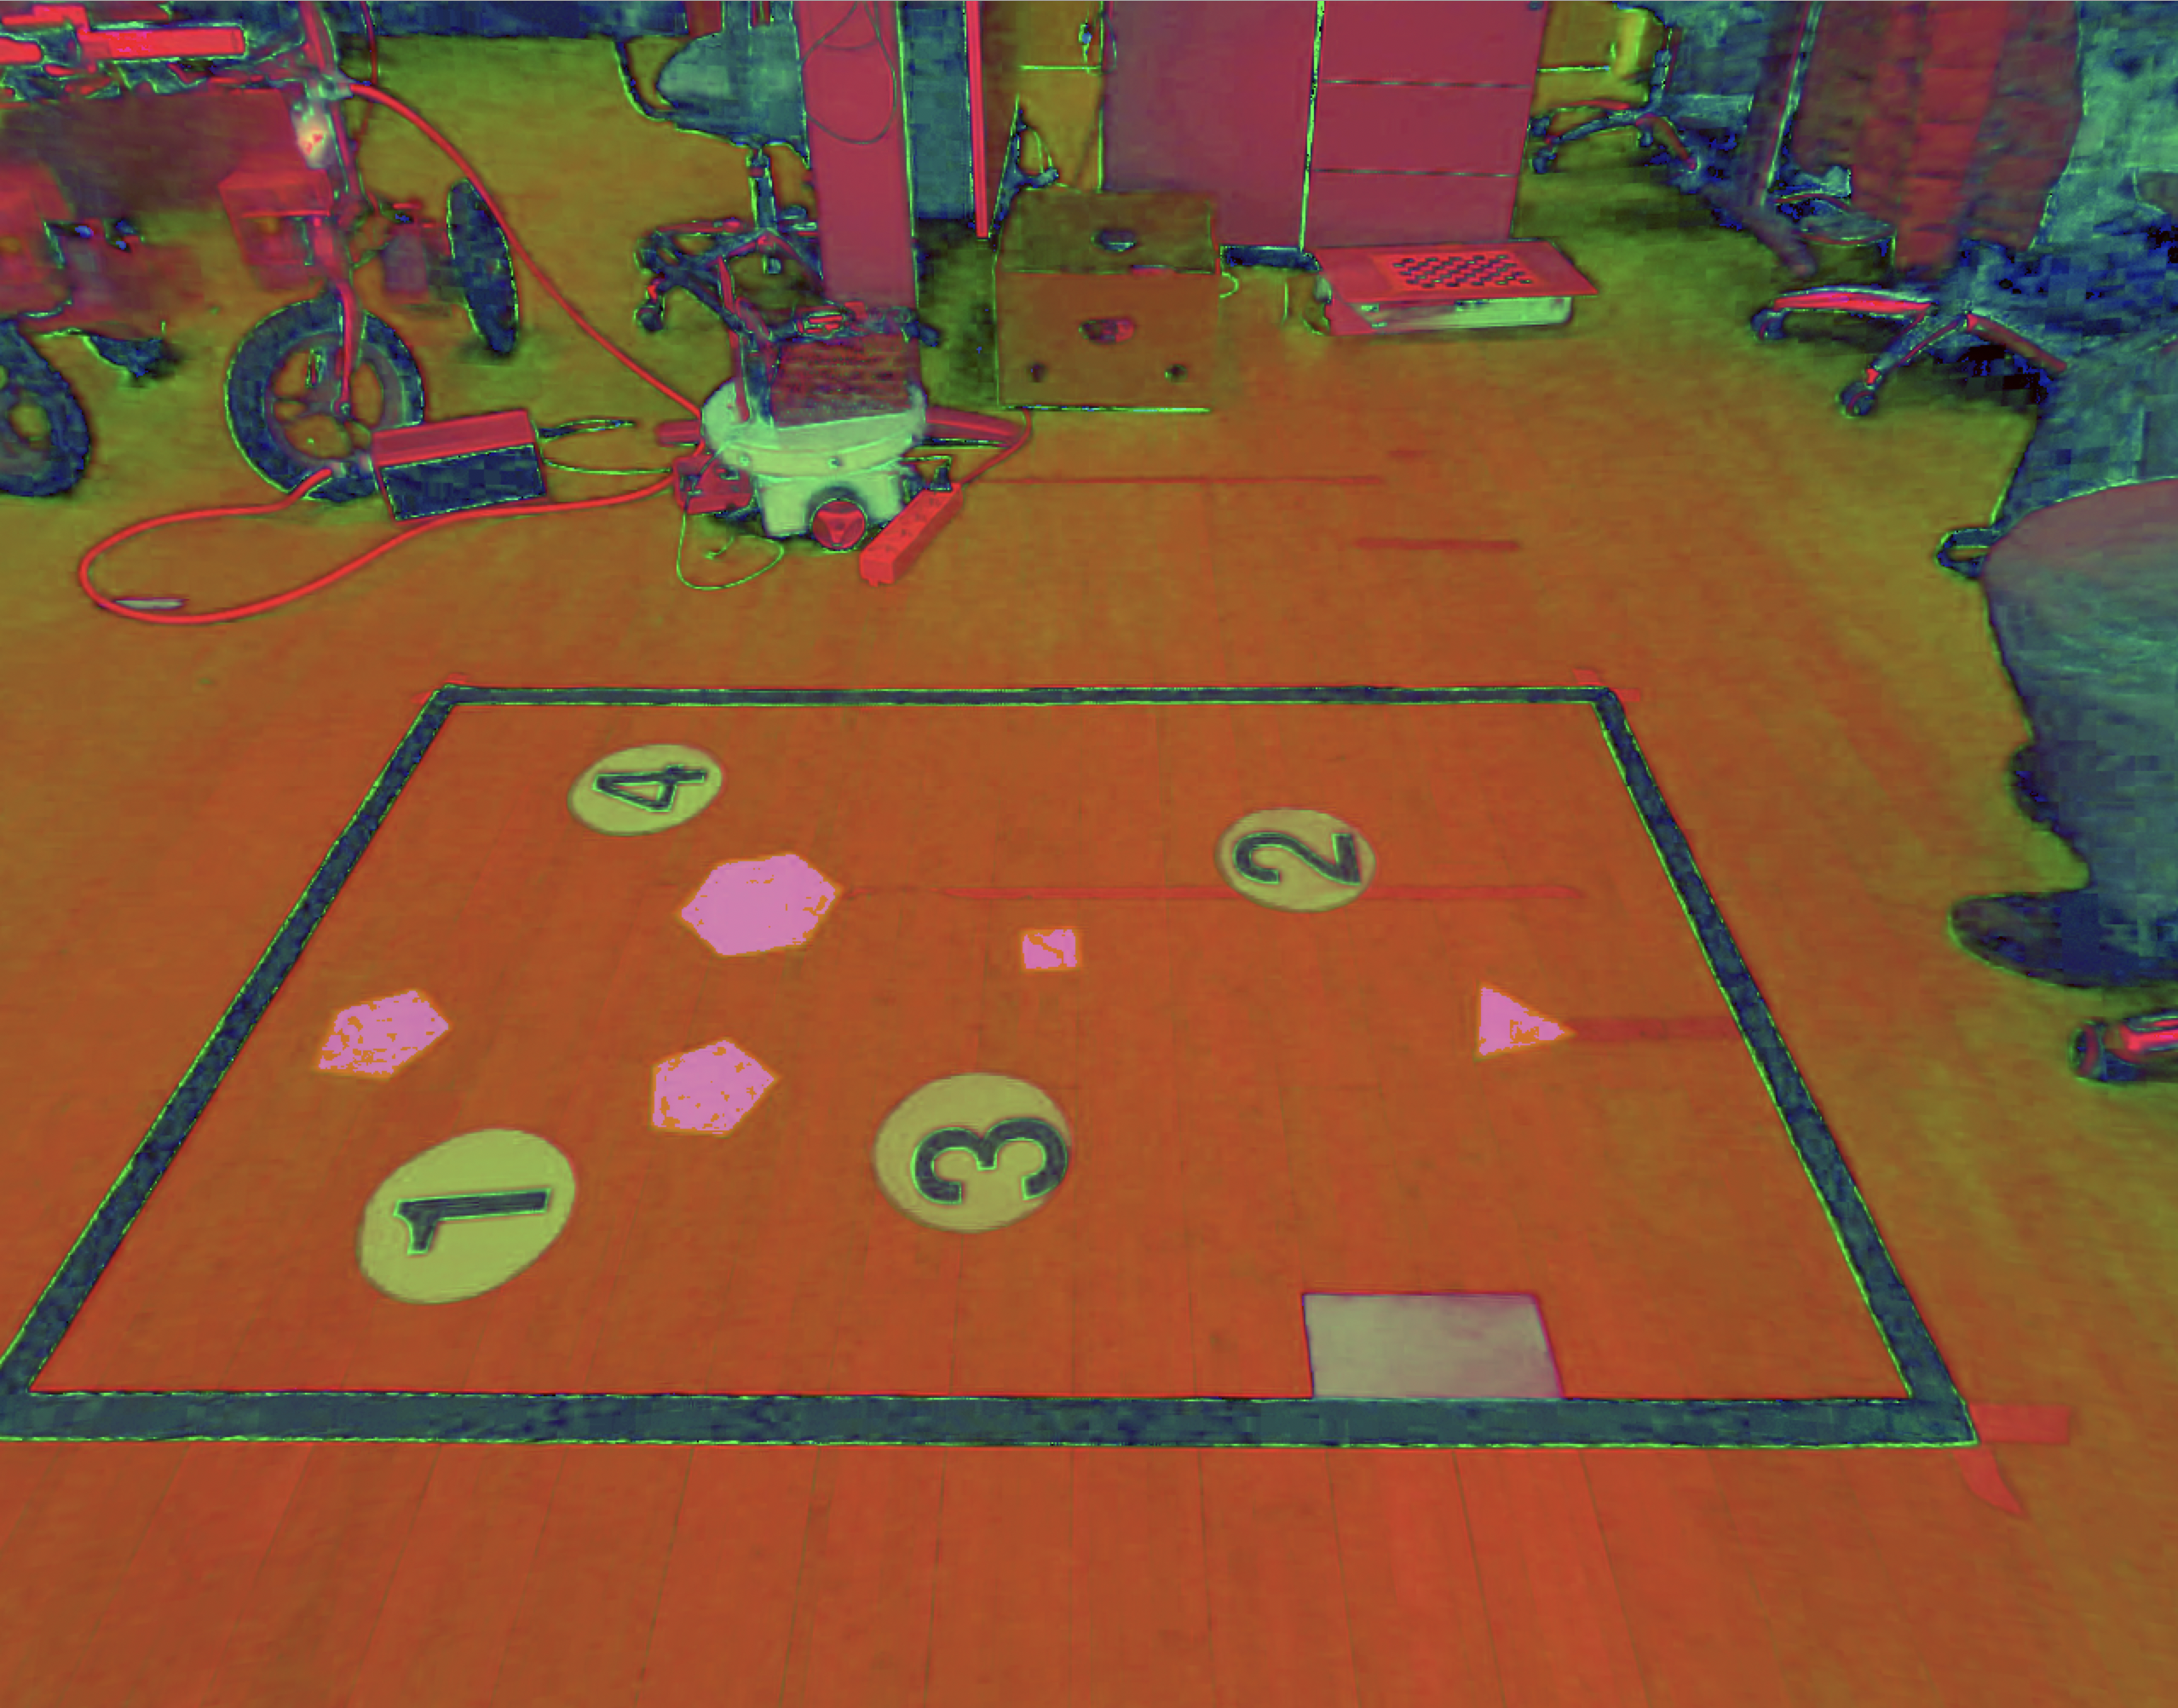
\includegraphics[scale=0.15]{Immagini/UNHSV}
	\end{center}
	\vfill
	\begin{minted}[fontsize=\stsize]{c++}
		cvtColor(fix_img, hsv_img, COLOR_BGR2HSV);
	\end{minted}
	\vfill
\end{frame}

\begin{frame}[fragile]{Unwarping}
	A black filter is added to highlight the black lines and areas.
	\begin{center}
		\includegraphics[scale=0.15]{Immagini/UNBlackFilter}
	\end{center}
	\vfill	
	\begin{minted}[fontsize=\stsize]{c++}
		Filter blackFilter = sett->blackFilter; 
        inRange(hsv_img, blackFilter.low(), blackFilter.high(), black_mask);
	\end{minted}
	\vfill
\end{frame}

\begin{frame}[fragile]{Unwarping}
	Then the largest area enclosed by black lines is selected. 
	\begin{center}
		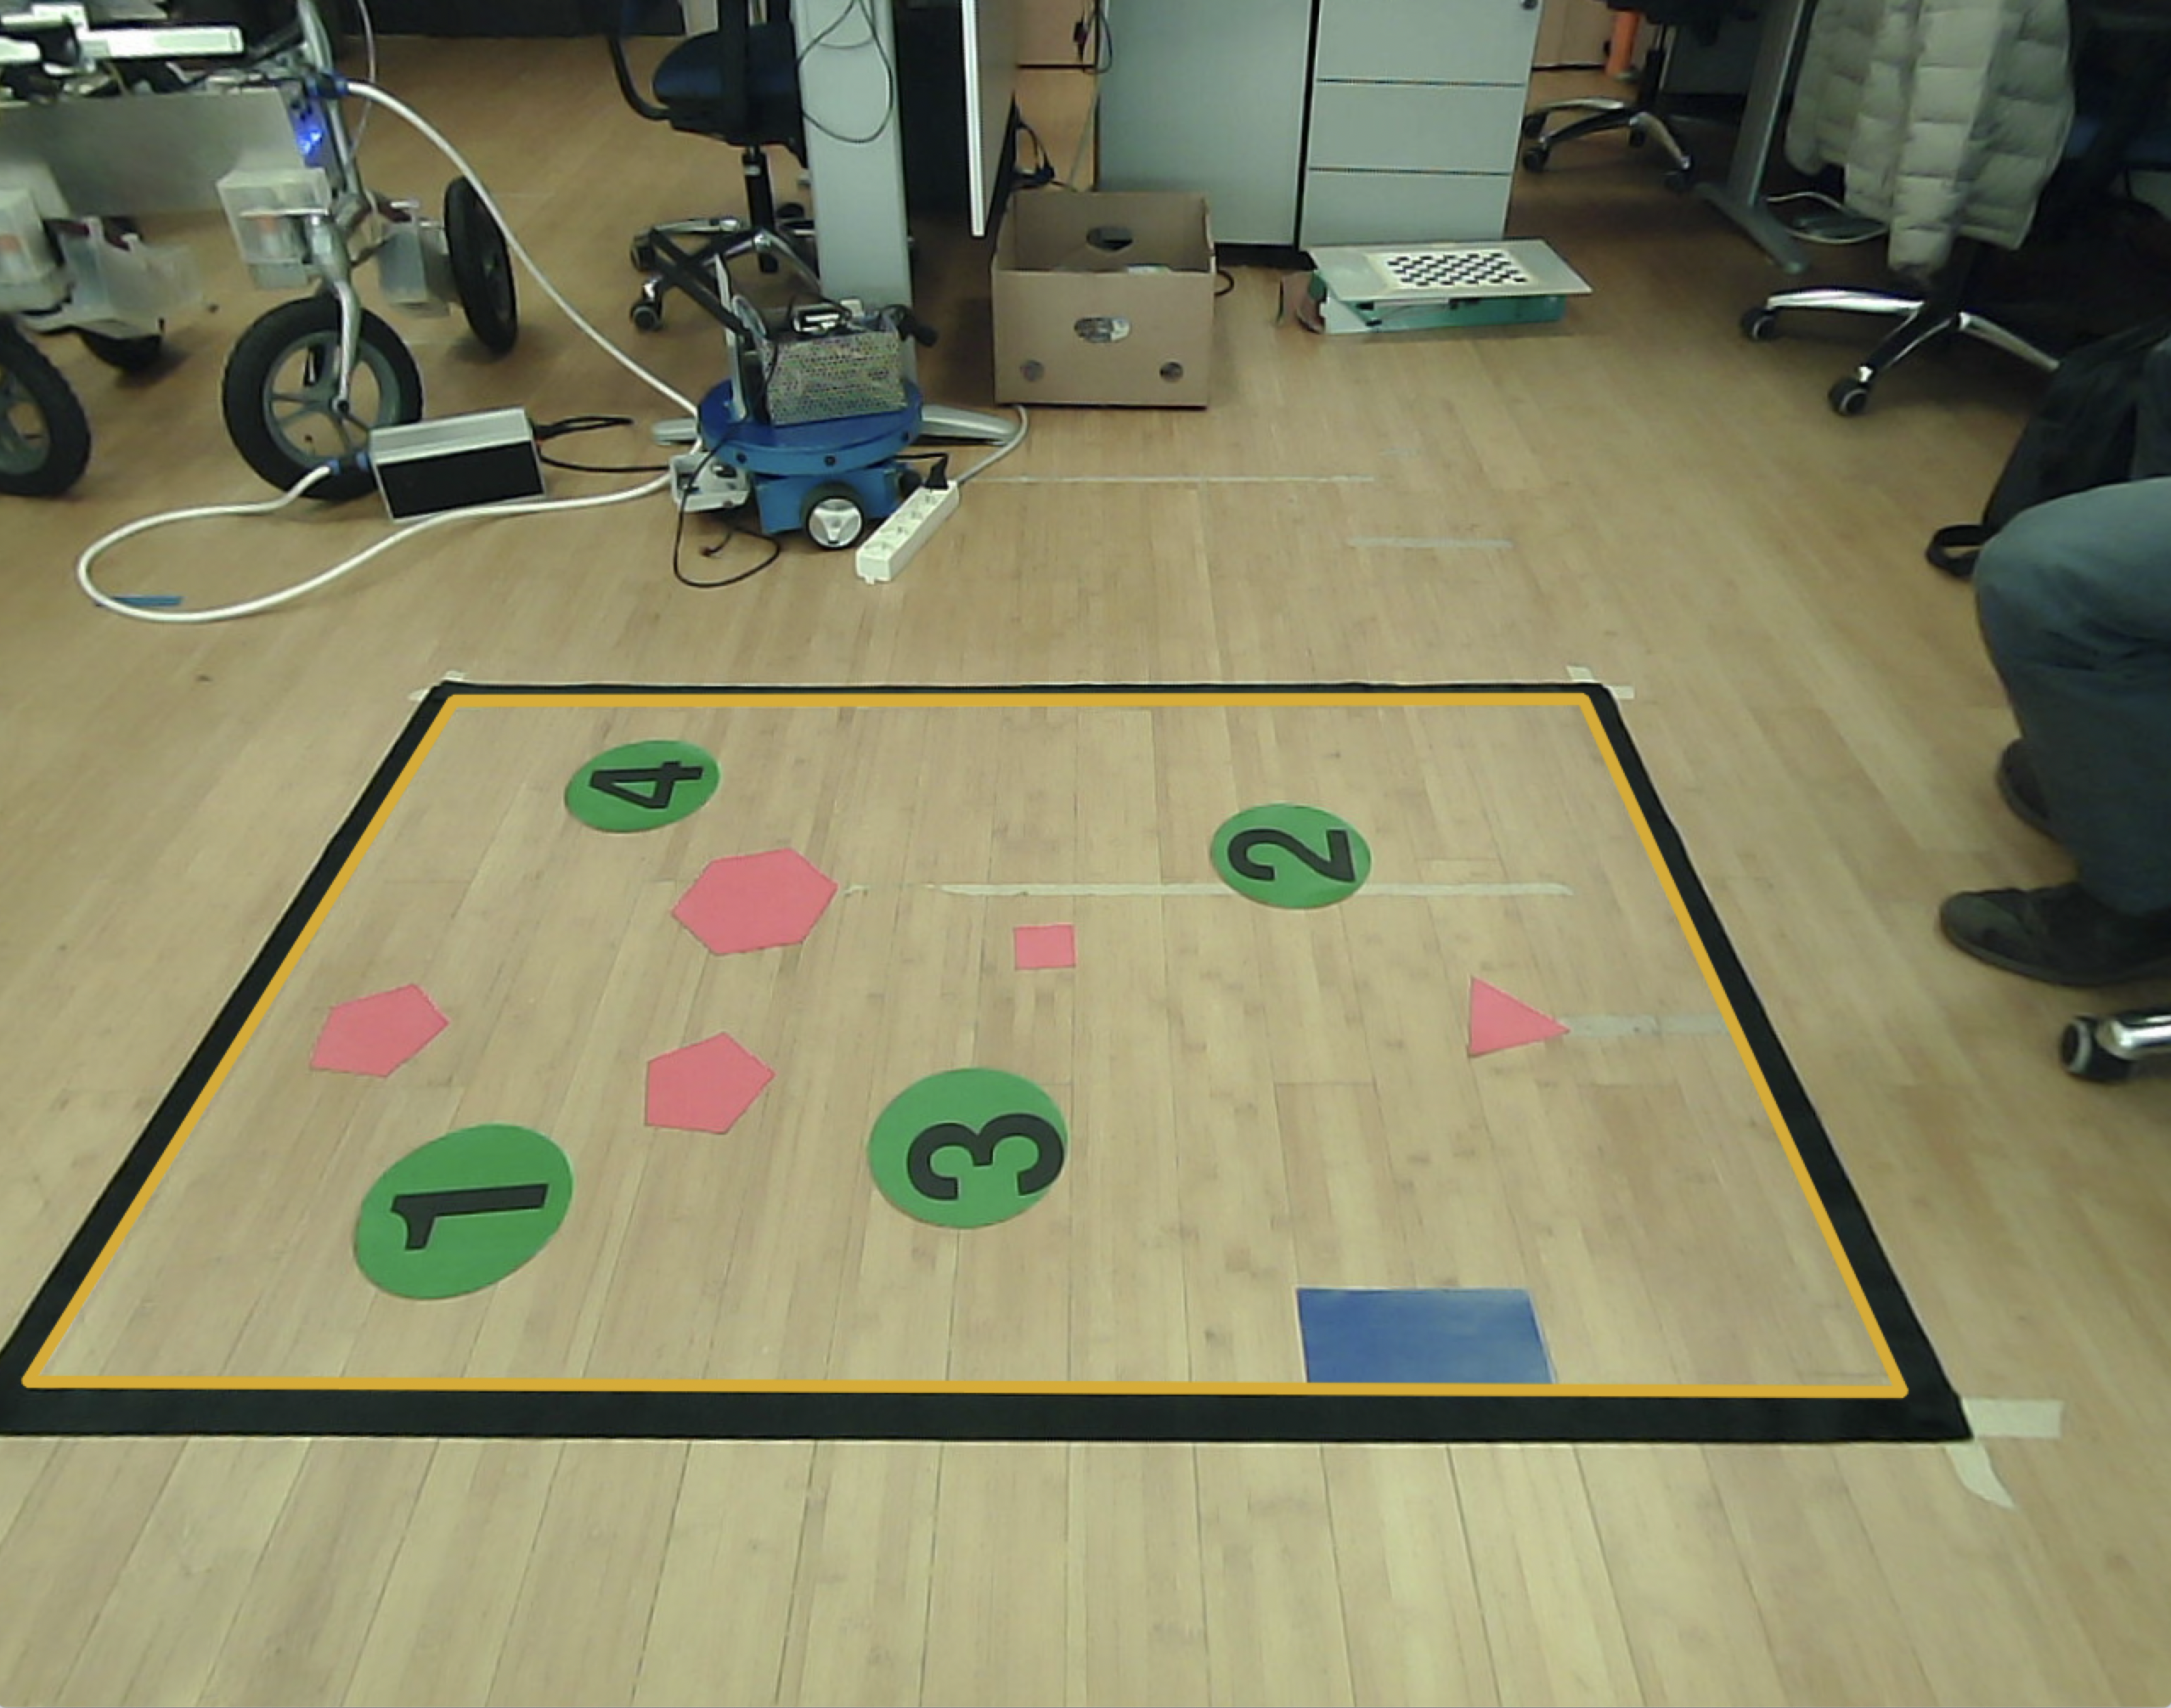
\includegraphics[scale=0.16]{Immagini/UNRect}
	\end{center}
\end{frame}

\begin{frame}[fragile]{Unwarping}
	At the end the image is cropped and turned. 
	\begin{center}
		\includegraphics[scale=0.18]{Immagini/Unwrapped.png}
	\end{center}
\end{frame}


\begin{frame}[fragile]{Detection}
	The detection phase consists of three more steps:
	\begin{itemize}
		\item Shape detection;
		\item Digit detection;
		\item Robot detection (aka localize).
	\end{itemize}
\end{frame}

\begin{frame}[fragile]{Shape detection}
\begin{figure}[H]
	\begin{minipage}{0.45\linewidth}
		The shape detection consists of scanning the image to locate the various obstacles, targets and the arriving point. \newline
		The various items are going to be stored in a file with the coordinates of their vertexes as convex hull. 
	\end{minipage}
	\vspace{0.07\linewidth}
	\begin{minipage}{0.48\linewidth}
		\includegraphics[width=\linewidth]{Immagini/all_detect}
	\end{minipage}
\end{figure}
\end{frame}


\begin{frame}[fragile]{Digit detection}
The goal of this phase is to consider the area around the targets, which is our ROI, and try to identify the number inside it. \newline
In order to have better results the area around each target is:
\begin{itemize}
	\item Cropped;
	\item Resized to $200$ $px\times 200$ $px$;
	\item Given a black filter thought for the victim;
	\item Passed through a function (\mintinline{c++}{erode_dilation()}) which aims at removing noise and isolating the number;
\end{itemize}
At last the digit detection is done with templates since the success rate has been greater than using Tesseract.
\end{frame}

\begin{frame}[fragile]{Number templates}
	\begin{figure}[H]
		\begin{minipage}{0.40\linewidth}
			\includegraphics[width=\linewidth]{Immagini/2.png}
		\end{minipage}
		\vspace{0.20\linewidth}
		\begin{minipage}{0.40\linewidth}
			\includegraphics[width=\linewidth]{Immagini/2_inv.png}
		\end{minipage}
	\end{figure}
\end{frame}

\begin{frame}[fragile]{Digit recognition}
\begin{center}
	\includegraphics[width=\linewidth]{Immagini/nn2}\\
	\includegraphics[width=\linewidth]{Immagini/nn3}
\end{center} 
\end{frame}

\begin{frame}[fragile]{Digit recognition}
\begin{center}
	\includegraphics[width=\linewidth]{Immagini/nn4}\\
	\includegraphics[width=\linewidth]{Immagini/nn5}
\end{center} 
\end{frame}

\begin{frame}[fragile]{Robot detection aka localize}
The barycentre of the robot is calculated as the mean of the \textit{hopefully} three vertexes of the triangle. \newline
The function is pretty fast since it works constantly under $20ms$. 
\begin{center}
	\includegraphics[scale=0.25]{Immagini/robot_detection}	
\end{center}
\end{frame}

\begin{frame}[fragile]{Robot detection aka localize}
Since the robot is not on the same plane as the arena, a first matrix transformation is needed to be able to use the same coordinates.  
\otsize
\[
\begin{bmatrix}
0.004009178727557017& 1.058423184075202& -85.87660834428323\\
-1.129379950738086& 0.01601083899628747& 1828.394707270977\\
-2.212284394884848e-05& 6.807241218637246e-06& \\	
\end{bmatrix}
\]
\begin{center}
\texttt{getPerspectiveTransform(...);}
\end{center}
\end{frame}

\begin{frame}{Map creation}
Map is represented as a matrix of cells. Each cell can be of 5 different types:
\begin{itemize}
	\item FREE
	\item VICT
	\item OBST
	\item GATE
	\item BODA
\end{itemize}
Each cell gets their type at the creation of the map by loading objects from file and then eventually applying an offset to the obstacles in order to consider the robot as a point.\newline
\href{https://icosac.github.io/LabRoboticsProject/html/map_8hh.html}{Link to map.hh}
\end{frame}

\begin{frame}[fragile]{Map creation}
\begin{center}
	\includegraphics[scale=0.19]{Immagini/map0}
\end{center}
\end{frame}

\begin{frame}[fragile]{Path planning}
\begin{figure}[H]
	\begin{minipage}{0.5\linewidth}
Once the map is created, we look at it as a graph and then compute a BFS to connect the robot to the gate through the victims in the right order.\newline
Here the direction of the robot means nothing: the total minimum path is always the sum of distance between each couple of cells.\newline
The complexity of this algorithm is $O(N+N(2R+1))$ where $N$=nodes and $R$=range=3. 
	\end{minipage}
	\vspace{0.20\linewidth}
	\begin{minipage}{0.40\linewidth}
		\href{https://icosac.github.io/LabRoboticsProject/html/planning_8hh.html}{\includegraphics[scale=0.19]{Immagini/map00}}
	\end{minipage}
\end{figure}
\end{frame}

\begin{frame}[fragile]{Dubins}
Once a min path is been computed, then we try to smooth it by applying \href{https://icosac.github.io/LabRoboticsProject/html/dubins_8hh.html}{Dubins curves}. 
\begin{figure}[H]
	\begin{minipage}{0.45\linewidth}
		\includegraphics[scale=0.15]{Immagini/map000}
	\end{minipage}
	\vspace{0.10\linewidth}
	\begin{minipage}{0.45\linewidth}
		\includegraphics[scale=0.15]{Immagini/map1}
	\end{minipage}
\end{figure}
\end{frame}

\begin{frame}[fragile]{Dubins}
\begin{figure}[H]
	\begin{minipage}{0.45\linewidth}
		\includegraphics[scale=0.19]{Immagini/map2}
	\end{minipage}
	\vspace{0.10\linewidth}
	\begin{minipage}{0.45\linewidth}
		\includegraphics[scale=0.19]{Immagini/map3}
	\end{minipage}
\end{figure}
\end{frame}

\begin{frame}[fragile]{Dubins}
\begin{figure}[H]
	\begin{minipage}{0.45\linewidth}
		\includegraphics[scale=0.19]{Immagini/map4}
	\end{minipage}
	\vspace{0.10\linewidth}
	\begin{minipage}{0.45\linewidth}
		\includegraphics[scale=0.19]{Immagini/map5}
	\end{minipage}
\end{figure}
\end{frame}

\begin{frame}{Honorable mentions}
\begin{figure}[H]
	\begin{minipage}{0.45\linewidth}
		\includegraphics[scale=0.13]{Immagini/map6}
	\end{minipage}
	\vspace{0.10\linewidth}
	\begin{minipage}{0.45\linewidth}
		\includegraphics[scale=0.13]{Immagini/map7}
	\end{minipage}
\end{figure}
\end{frame}

\begin{frame}{The bonus problem}
The robot can save (or not) the victims in any order, getting a prize for each rescue. \newline
To do this, the min path algorithm has been changed:
\begin{itemize}
	\item It computes the distances between each couple of elements as a complete graph.
	\item It try all the possible combinations of routes considering the bonus.
	\item Finally choose the cheapest combination and apply Dubins. 
\end{itemize}
\end{frame}

\begin{frame}{Known problem}
\begin{figure}[H]
	\begin{minipage}{0.45\linewidth}
A known problem is what we called "The tunnel problem".\newline
This problem is due to the fact that the min path algorithm does not consider directions and the sample algorithm of the Dubins cannot always find a solution.  
	\end{minipage}
	\vspace{0.10\linewidth}
	\begin{minipage}{0.45\linewidth}
		\includegraphics[scale=0.13]{Immagini/polmoni}
	\end{minipage}
\end{figure}
\end{frame}

\begin{frame}{Acknowledgments}
\begin{center}
Thank you for your attention. 
\end{center}
\end{frame}

